%-------------------------------------------------------------------------------
\section{Problem}\label{s:problem}
%-------------------------------------------------------------------------------

The observed failure to protect the server application's reservation from the
image resize job happens because the latter sometimes runs uncontended on one
core, even while another has queued and waiting server threads
(\autoref{ss:problem:bes-run}). This is because weights are only strictly
enforced within runqueues, which are per-CPU
(\autoref{ss:problem:weights-local}). Weights are complicated and expensive to
enforce across cores (\autoref{ss:problem:cross-core-hard}), as well as
interacting poorly with Linux's large scheduling quantum
(\autoref{ss:problem:quantum}).

\subsection{Weights are a local property}\label{ss:problem:bes-run}

\begin{figure}[t]
    \centering
    \begin{subfigure}{\columnwidth}
        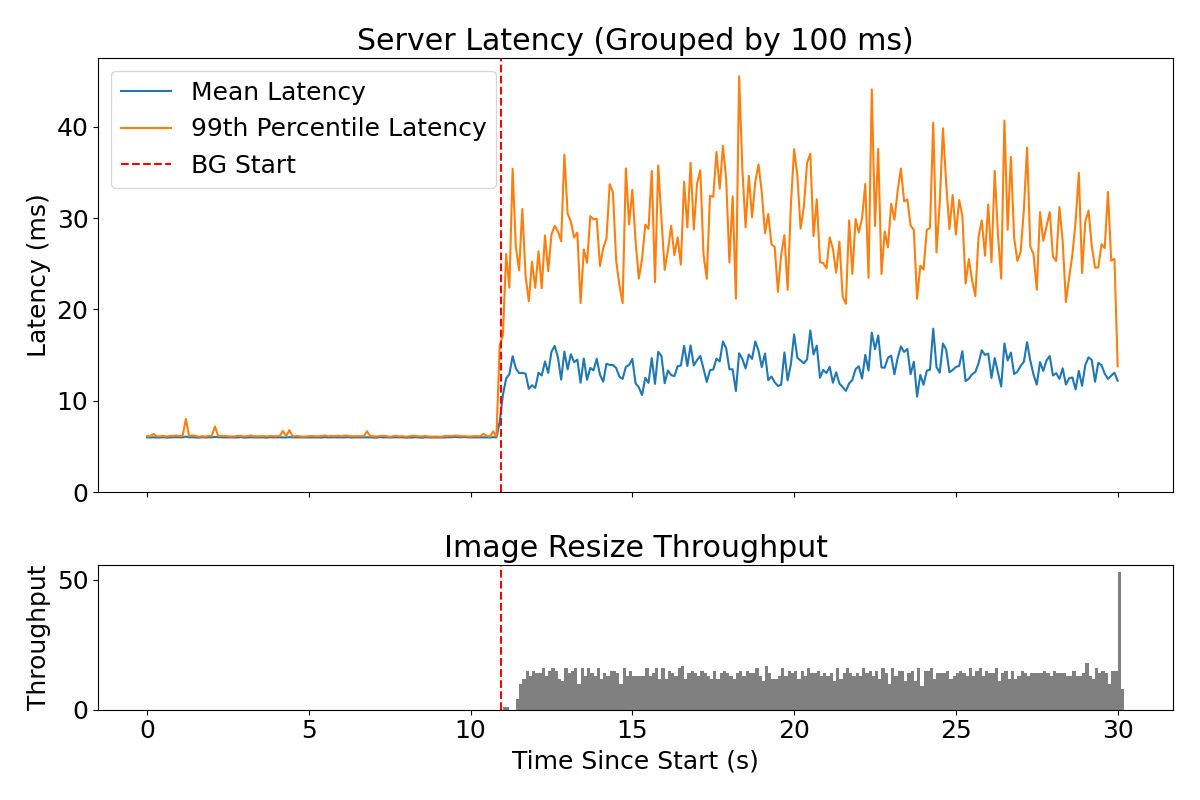
\includegraphics[width=\columnwidth]{graphs/srv-bg-weight-low.png}
        \caption{Low load stetting, utilization before starting the BE tasks is
        around 85\%}\label{fig:srv-bg-weight-low}
        \vspace{12pt}
    \end{subfigure}
    \hspace{\fill}
    \begin{subfigure}{\columnwidth}
        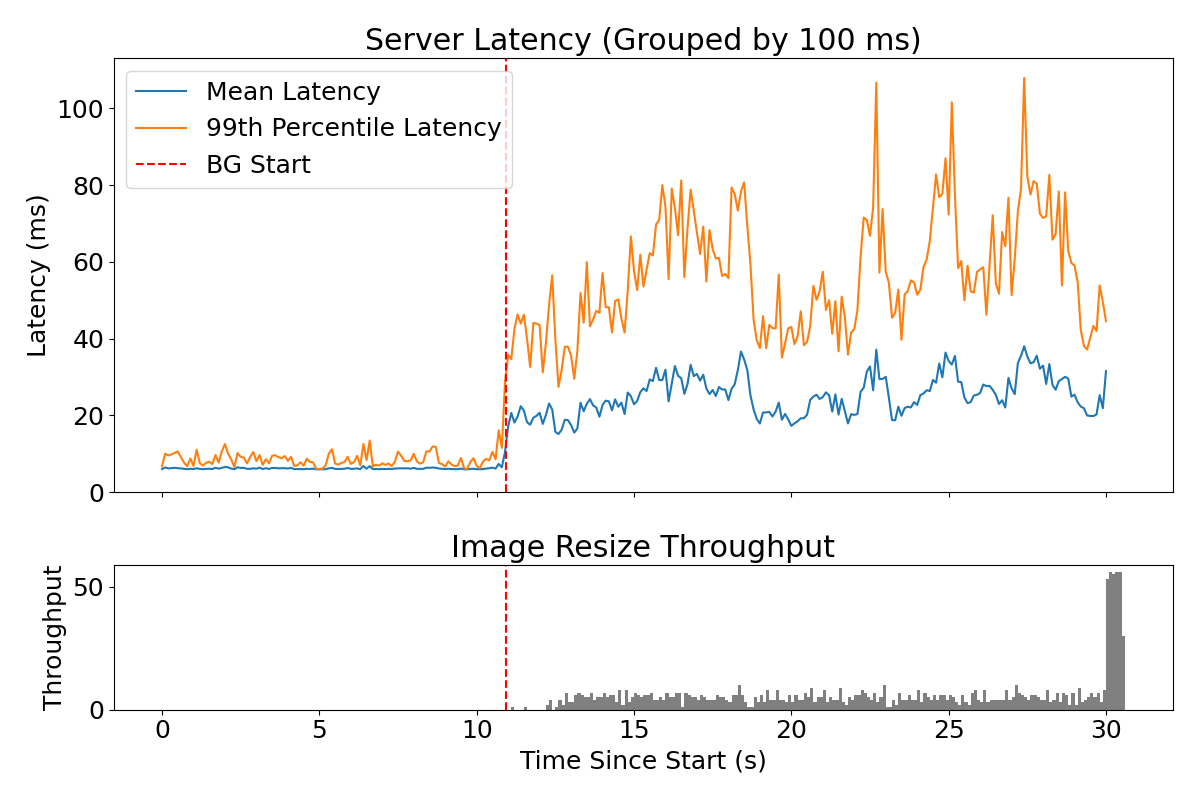
\includegraphics[width=\columnwidth]{graphs/srv-bg-weight-high.png}
        \caption{High load setting, utilization before starting the BE tasks is
        around 95\%}\label{fig:srv-bg-weight-high}
    \end{subfigure}
    \vspace{4pt}
    \caption{in a simplified experiment using \cgroups{}, running best effort
    tasks has a large impact on the latency critical
    server}\label{fig:srv-bg-weight}
\end{figure}

In order to understand why the jump in latency is happening when the best effort
task runs, we reproduce the effects in a simpler benchmark. The experiment shown
in \autoref{fig:kubernetes-unedited} includes a complicated software stack of
Kubernetes, uvicorn, FastAPI, and Python. All of this has performance
implications, and we can see that even before the image resize job starts there
are large latency spikes up to 30ms.

To exclude these effects, we run a simple CPU-bound server with a pool of worker
threads. We run an open-loop client on a remote machine, and then start two best
effort workloads doing image resizing. We put the LC server and the BE resize
job each in their own \cgroups{} group with weights 150 and 1 respectively
(similar to Kubernetes), and pin them to the same set of four cores.

\autoref{fig:srv-bg-weight} shows the result: we see that at a $\sim$85\%
baseline utilization of the server, after starting the image resize jobs the
server's mean latencies spike up from steady at around 6ms to $\sim$15ms, and
much higher for 99th percentile latencies. At a baseline utilization of 95\%,
those numbers increase to up to 40ms for the the mean latency, and 80ms for the
tail.

\begin{figure}[t]
    \centering
    \begin{subfigure}{\columnwidth}
        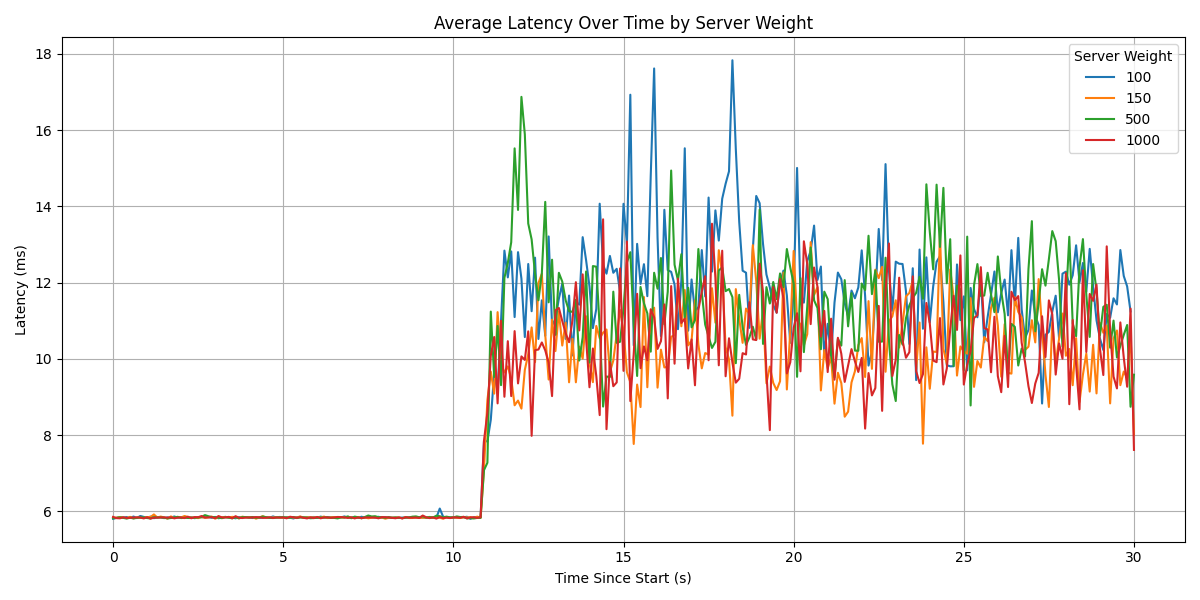
\includegraphics[width=\columnwidth]{graphs/srv-bg-weight-cmp-low.png}
        \caption{Low load stetting, utilization before starting the BE tasks is
        around 85\%}\label{fig:srv-bg-weight-cmp-low}
        \vspace{12pt}
    \end{subfigure}
    \hspace{\fill}
    \begin{subfigure}{\columnwidth}
        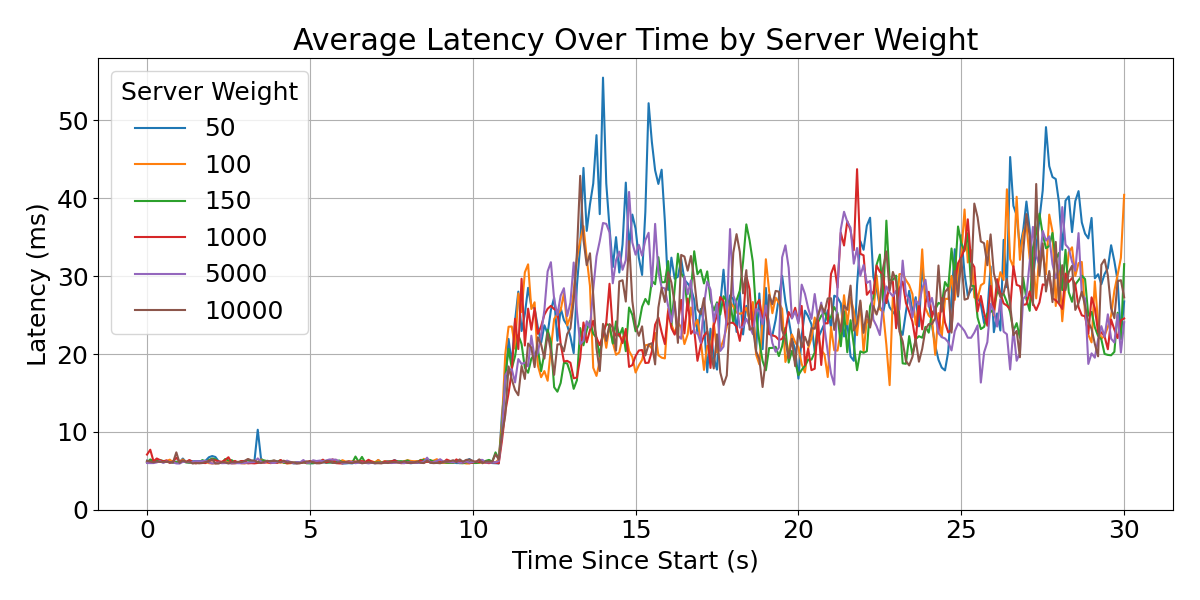
\includegraphics[width=\columnwidth]{graphs/srv-bg-weight-cmp-high.png}
        \caption{High load setting, utilization before starting the BE tasks is
        around 95\%}\label{fig:srv-bg-weight-cmp-high}
    \end{subfigure}
    \vspace{4pt}
    \caption{Changing the weight of the server beyond 100 has little impact on
    how much the weight 1 best effort task interferes with it}\label{fig:srv-bg-weight-cmp}
\end{figure}

\cgroups{} supports weights in the range of [1,10000]; a possible explanation
could be that Kubernetes did not set the weights far apart enough. Running the
same experiment with the server weight set to different values shows that using
a bigger weight split has no impact on the latency impact of the best effort
task. \autoref{fig:srv-bg-weight-cmp} shows the average server latencies when
running it with different weights; the image resize task always has weight 1.

\begin{figure}[t]
    \centering
    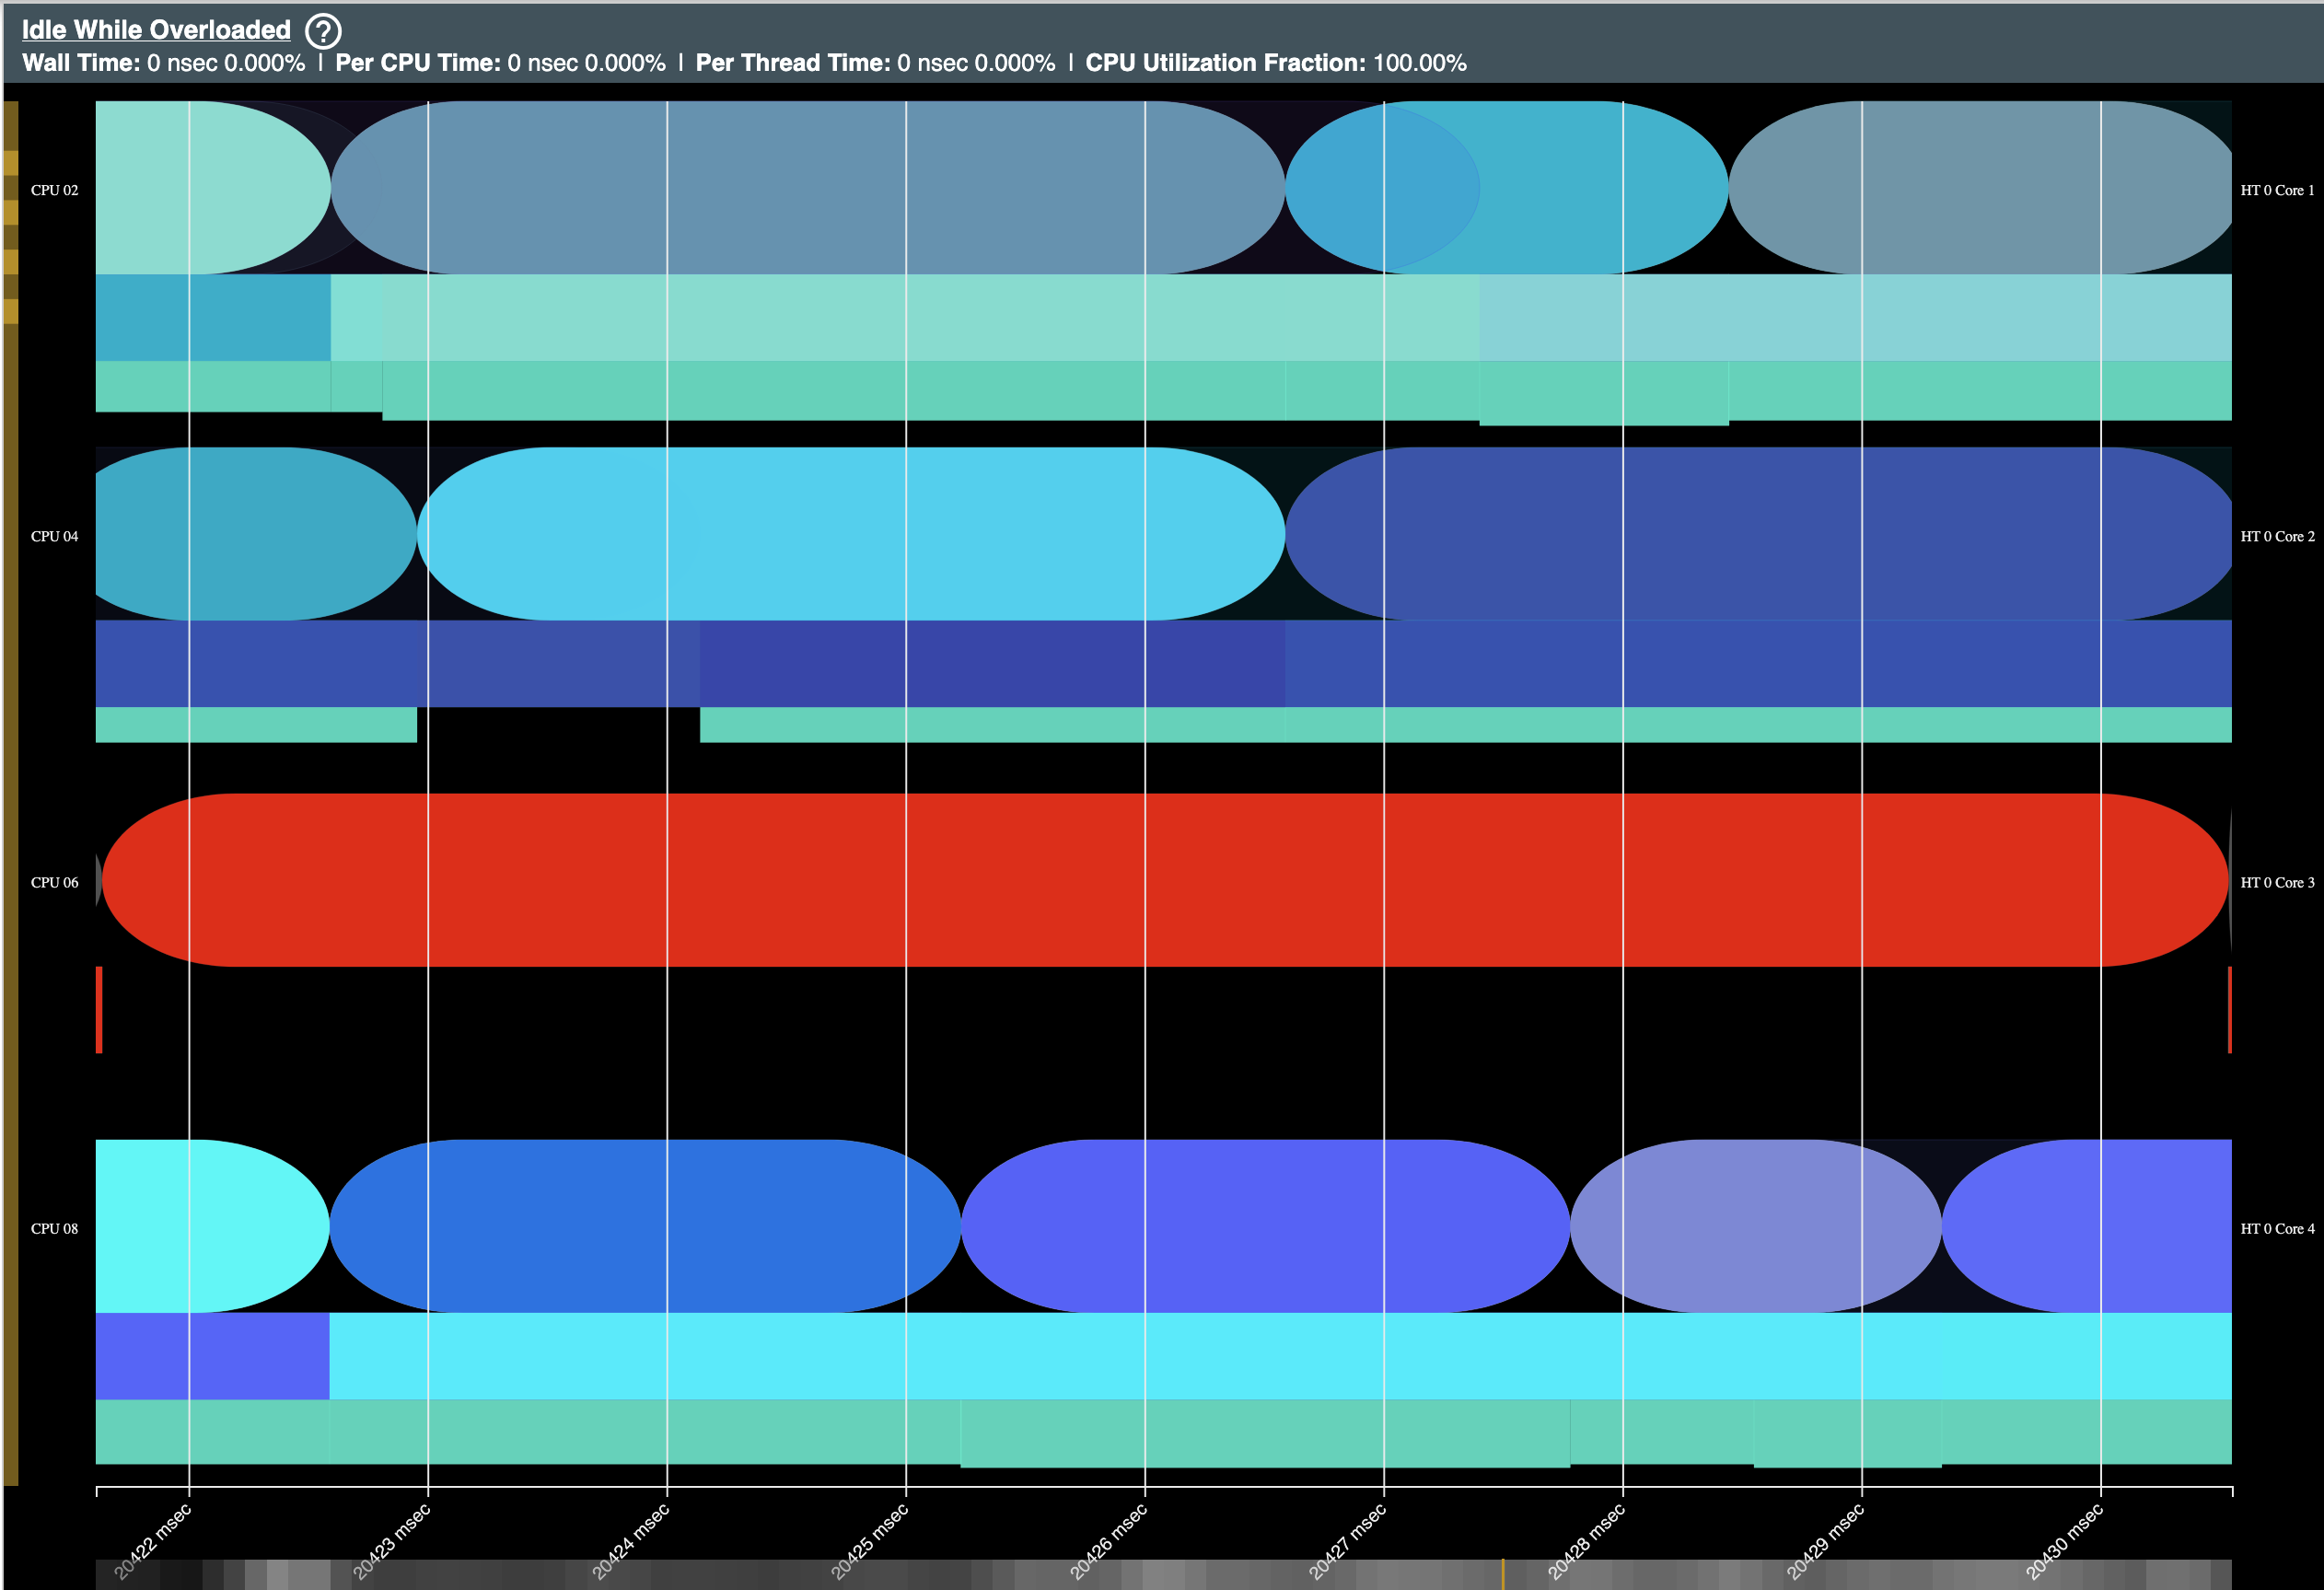
\includegraphics[width=\columnwidth]{graphs/schedviz-problem.png}
    \caption{Core 6 runs an image resize process, unaware that cores 2, 4, and 8
    all have runnable and queued server threads}\label{fig:schedviz-problem}
\end{figure}

For this simplified experiment we analyze perf traces of the scheduling
decisions by visualizing the trace using schedviz~\cite{schedviz-tool}.
\autoref{fig:schedviz-problem} shows a 10ms outtake of the resulting image. The
process running on each core is shown as an oval, and queued processes are shown
as rectangles below; the x-axis is time and the y-axis shows the 4 cores the
experiment is running on. What we see is that \textit{one core is running a best
effort process, while threads of processes with resource reservations are queued
on another}. On core 6, the red process that is running for the whole 10ms is a
thread of the image resize job, while server threads, shown in varying shades of
blue, are queued on the other cores.

\subsection{Weights are enforced only locally}\label{ss:problem:weights-local}

The reason this priority inversion is possible is that Linux maintains a
separate runqueue on each core, in order to avoid the overheads of accessing
global state for every scheduling decision. Within each runqueue, Linux's
scheduler works to maintain the correct ratio of received CPU time at each
scheduling; but Linux does not enforce the weight ratios across cores. 

The threading model of the server interacts with the per-core runqueues. The
server uses a pool of worker threads (one per client). The number of threads
that the server has is larger than the number of cores, which means that each
core has multiple server threads. It occasionally occurs that all the current
requests are on server threads that happen to be on only three of the four
available cores, which leaves one runqeueue with only idle server worker
threads. Although load balancing eventually remedies this, load balancing runs
less frequently than scheduling does, at least during high load: how often load
balancing runs in general is a complicated number that is dependent on how close
the two cores are in the CPU architecture hierarchy, as well as how loaded the
machine is.

This leads to the above failure mode, where one core has no runnable high weight
server threads and thus runs a low weight one, while other cores have queued
high weight processes.

\subsection{Enforcing weights across cores is
hard}\label{ss:problem:cross-core-hard}

A weight-based interface is at odds with machine-wide policy enforcement. In
order to globally enforce a processes weight, the scheduler would need to
look at every cores' runqueues at every scheduling decision. 

This check needs to happens at every tick because, in a weight-based system, the
definition of what process should be running changes over time. If a core has
one high-weight and one low-weight group, before running the low-weight group it
needs to know if any other cores have recently run a different process within
that group, because that would affect how much time it is owed on this core.

Enforcing weights across cores is expensive: looking at remote queues at each
scheduling decision removes the benefit of having local runqueues. Inter-core
communication and having every core look at every other cores' runqueues can
lead to contention, which has been demonstrated to be a bottleneck for
performance at scale~\cite{afaas}. This means that the overheads of maintaining
a weight split as a global invariant can quickly become prohibitive.

On top of the communication cost, managing and calculating global shares is
complex: calculating whether a given process is owed time globally requires
knowing the total weight across all cores as well as the sum of time that all
the processes in the group have gotten. Such a calculation would include
complicated accounting that takes into account, amount other things, different
cores' virtual times, processes' weights, groups, and limits. Just within
runqueues the accounting is already so complicated that comments in the Linux
source include function derivations and equation rewriting.


\subsection{Weights interact poorly with tick-based
scheduling}\label{ss:problem:quantum}

Even on a single runqueue, in a weight based scheme best effort processes need
to get a fair share of the CPU. The problem is that, when this happens, the BE
process will interrupt any running LC process for a whole tick. In Linux,
hardware ticks are 4ms long. This means that a thread that has a CPU reservation
and is processing a request may be interrupted for up to 4ms by a best effort
process, provided the latter runs that long before blocking. 4ms can be a large
amount of time for microservice workloads, whose SLOs are often in the low
double digit or even single digit ms realm.~\cite{in-the-plex, sigmaos}



